\documentclass{article}
\usepackage{graphicx} % Required for inserting images
\usepackage{amsmath}  % Required for advanced math environments like align*
\usepackage{amssymb}  % For more math symbols
\usepackage{amsfonts}
\usepackage{pdfpages}
\usepackage{enumitem} % For custom lists

% --- GEOMETRY PACKAGE FOR PAGE LAYOUT ---
\usepackage[
    left=1in,
    textwidth=6.5in, 
    top=1in,
    bottom=1in
]{geometry}
% -----------------------------------------

\title{Chapter 5 Quiz - Revision}
\author{Tashfeen Omran}
\date{September 2025}

\begin{document}

\maketitle
\pagenumbering{gobble} % Removes page numbering


\hrulefill
\subsection*{Quiz Details:}
\begin{itemize}[itemsep=5pt]
    \item \textbf{When:} Tuesday, September 23rd, 7:00 AM - 7:30 AM.
    \item \textbf{Format:} Closed notes.
    \item \textbf{Allowed Materials:} A clean, unmarked copy of the "Periodic Table for testing" PDF.
\end{itemize}

\hrulefill
\subsection*{Key Topics:}
\begin{itemize}[itemsep=5pt]
    \item \textbf{Lattice Energy:} Ranking ionic compounds.
    \item \textbf{Nomenclature:} Naming and writing formulas for ionic and molecular compounds.
    \item \textbf{Empirical Formulas:} Calculating the empirical formula from percent composition.
\end{itemize}
\hrulefill
\bigskip
\subsection*{Phase 1: Foundation (Friday/Saturday)}
\begin{itemize}[itemsep=5pt]
    \item \textbf{Core Concepts Review:} Carefully read through the "Chapter 5 Ionic and Covalent Compounds.pdf" PowerPoint presentation. Pay special attention to these slides:
    \begin{itemize}
        \item \textbf{Slides 7-14:} Understand what lattice energy is and the two factors that affect it (ionic charge and atomic radius).
        \item \textbf{Slides 17, 19:} Master the rules for naming ionic compounds and using Roman numerals for transition metals.
        \item \textbf{Slides 22-24:} Learn the rules for naming binary molecular (covalent) compounds using Greek prefixes.
        \item \textbf{Slide 56:} Understand the concept of an empirical formula.
    \end{itemize}
    \item \textbf{Memorize Polyatomic Ions:} Use Slide 36 ("Polyatomic ions you should know by heart") to create flashcards. You must know these names, formulas, and charges. This is crucial for ionic nomenclature.
\end{itemize}

\bigskip
\subsection*{Phase 2: Practice \& Application (Sunday)}
\begin{itemize}[itemsep=5pt]
    \item \textbf{Nomenclature Drills:}
    \begin{itemize}
        \item Take out a blank piece of paper and work through all the problems in the "Ionic nomenclature practice Answer Key.pdf". Try to answer first before checking the key.
        \item Do the same for the covalent compounds only in "Covalent, hydrate, and acid nomenclature Answer Key.pdf". (Remember, acids and hydrates are not on this quiz).
    \end{itemize}
    \item \textbf{Lattice Energy Ranking:}
    \begin{itemize}
        \item Review the examples on slides 12 and 14 of the PowerPoint.
        \item Without looking at the answers, try to rank the compounds and write down your reasoning (e.g., "MgO has a higher lattice energy than CaO because Mg$^{2+}$ is smaller than Ca$^{2+}$").
    \end{itemize}
\end{itemize}

\bigskip
\subsection*{Phase 3: Final Mastery (Monday)}
\begin{itemize}[itemsep=5pt]
    \item \textbf{Empirical Formula Calculations:}
    \begin{itemize}
        \item Review the step-by-step process on slides 57-63 of the PowerPoint.
        \item Work through every problem in the "Empirical and molecular formulae Answer Key.pdf". Focus on the process:
        \begin{itemize}
            \item Percent to Mass (assume 100g)
            \item Mass to Moles (use molar mass)
            \item Divide by Smallest Mole Value
            \item Make it a Whole Number Ratio (multiply if necessary)
        \end{itemize}
        \item Pay close attention to the rule about not rounding numbers like 1.5, 1.33, etc.
    \end{itemize}
    \item \textbf{Final Review \& Prep:}
    \begin{itemize}
        \item Briefly review all topics again. The flowchart on Slide 42 is an excellent summary for nomenclature.
        \item Print a clean copy of the "Periodic Table for testing" PDF. Make sure it has no writing on it.
        \item Get a good night's sleep.
    \end{itemize}
\end{itemize}

\bigskip
\section*{Explanations of Practice Problems}
Below are detailed walkthroughs of the questions from your provided files, focusing only on the topics relevant to your quiz.

\subsection*{Topic 1: Lattice Energy}
This concept is covered in the "Chapter 5 Ionic and Covalent Compounds.pdf" PowerPoint.

\subsubsection*{Key Principles (Slides 8, 11-14):}
Lattice energy is the energy that holds an ionic crystal together. To rank it, follow two rules in order:
\begin{enumerate}[itemsep=5pt]
    \item \textbf{Ionic Charge:} The larger the charges of the ions, the stronger the attraction and the higher the lattice energy. A compound with +2 and -2 ions will have a much higher lattice energy than one with +1 and -1 ions. This is the most important factor.
    \item \textbf{Ionic Radius (Size):} If the charges are the same, smaller ions lead to a higher lattice energy because they can get closer together, making the electrostatic attraction stronger. Use the periodic table trend: ions get larger as you go down a group.
\end{enumerate}

\subsubsection*{Example 1: Arrange AlN, NaCl, and MgI$_2$ in order of increasing lattice energy. (from Slide 12)}
\begin{enumerate}[label=Step \arabic*:, itemsep=5pt]
    \item \textbf{Identify the ion charges.}
    \begin{itemize}
        \item NaCl $\rightarrow$ Na$^{+}$ and Cl$^{-}$ (+1, -1)
        \item MgI$_2$ $\rightarrow$ Mg$^{2+}$ and I$^{-}$ (+2, -1)
        \item AlN $\rightarrow$ Al$^{3+}$ and N$^{3-}$ (+3, -3)
    \end{itemize}
    \item \textbf{Compare charges.} The magnitudes of the charges are ($1 \times 1=1$) for NaCl, ($2 \times 1=2$) for MgI$_2$, and ($3 \times 3=9$) for AlN.
    \item \textbf{Rank based on charge.} Since charge is the dominant factor, the order of increasing lattice energy is directly related to the magnitude of the charges.
\end{enumerate}
\textbf{Answer:} NaCl $<$ MgI$_2$ $<$ AlN

\subsubsection*{Example 2: Arrange MgO, SrO, and CaO in order of increasing lattice energy. (from Slide 14)}
\begin{enumerate}[label=Step \arabic*:, itemsep=5pt]
    \item \textbf{Identify the ion charges.}
    \begin{itemize}
        \item MgO $\rightarrow$ Mg$^{2+}$ and O$^{2-}$ (+2, -2)
        \item CaO $\rightarrow$ Ca$^{2+}$ and O$^{2-}$ (+2, -2)
        \item SrO $\rightarrow$ Sr$^{2+}$ and O$^{2-}$ (+2, -2)
    \end{itemize}
    \item \textbf{Compare charges.} All the compounds have the same magnitude of charges (+2, -2). Therefore, we must use the second rule: ionic radius.
    \item \textbf{Compare radii of the cations.} Mg, Ca, and Sr are all in Group 2. Atomic radius increases as you go down the group. Therefore, the ionic size order is Mg$^{2+}$ $<$ Ca$^{2+}$ $<$ Sr$^{2+}$.
    \item \textbf{Rank based on radius.} Since lattice energy is inversely proportional to radius, the compound with the smallest cation (Mg$^{2+}$) will have the highest lattice energy.
\end{enumerate}
\textbf{Answer:} SrO $<$ CaO $<$ MgO

\bigskip
\subsection*{Topic 2: Ionic and Molecular Nomenclature}

\subsubsection*{Ionic Nomenclature (from "Ionic nomenclature practice Answer Key.pdf")}
\textbf{Rules:}
\begin{enumerate}[itemsep=5pt]
    \item The metal (cation) is named first, using its element name.
    \item If the metal is a transition metal that can have multiple charges (like Iron, Copper, Lead), its charge is written in Roman numerals in parentheses, e.g., Iron (II).
    \item The nonmetal (anion) is named second, with its ending changed to \textbf{-ide}.
    \item If the anion is a polyatomic ion, use its specific name (e.g., SO$_4^{2-}$ is "sulfate").
\end{enumerate}

\subsubsection*{Practice Problems Explained:}
\begin{itemize}[itemsep=5pt]
    \item \textbf{1a) Ca(NO$_3$)$_2$:} Ca is Calcium. NO$_3$ is the polyatomic ion nitrate. \textbf{Name: Calcium nitrate.}
    \item \textbf{1b) Li$_3$P:} Li is Lithium. P is Phosphorus, which becomes phosphide. \textbf{Name: Lithium phosphide.}
    \item \textbf{1c) AuBr$_3$:} Au is Gold. It's a transition metal. Bromine (Br) has a -1 charge. Since there are three Br ions, the total negative charge is -3. To balance this, the one Au ion must be +3. \textbf{Name: Gold (III) bromide.}
    \item \textbf{1d) CrS$_3$:} Cr is Chromium. Sulfur (S) is in group 16 and typically has a -2 charge. With three S ions, the total negative charge is -6. The one Cr ion must be +6 to balance. \textbf{Name: Chromium (VI) sulfide.}
    \item \textbf{5a) KBr:} K is Potassium. Br is Bromine, which becomes bromide. \textbf{Name: Potassium bromide.}
    \item \textbf{5b) FePO$_4$:} Fe is Iron. PO$_4$ is the phosphate ion, which has a -3 charge. To balance, the one Fe ion must be +3. \textbf{Name: Iron (III) phosphate.}
\end{itemize}

\subsubsection*{Covalent (Molecular) Nomenclature (from "Covalent, hydrate, and acid nomenclature Answer Key.pdf")}
\textbf{Rules:}
\begin{enumerate}[itemsep=5pt]
    \item The first element is named using its element name. Use a Greek prefix (di-, tri-, etc.) only if there is more than one atom of that element.
    \item The second element is named with its ending changed to \textbf{-ide}.
    \item The second element \textit{always} gets a Greek prefix (mono-, di-, tri-, etc.) to indicate the number of atoms.
\end{enumerate}

\subsubsection*{Practice Problems Explained:}
\begin{itemize}[itemsep=5pt]
    \item \textbf{1a) NBr$_3$:} N is Nitrogen. There are three (tri) Bromine atoms (bromide). \textbf{Name: Nitrogen tribromide.}
    \item \textbf{1b) S$_2$Cl$_4$:} There are two (di) Sulfur atoms. There are four (tetra) Chlorine atoms (chloride). \textbf{Name: Disulfur tetrachloride.}
    \item \textbf{1c) P$_2$S$_5$:} Two (di) Phosphorus atoms. Five (penta) Sulfur atoms (sulfide). \textbf{Name: Diphosphorus pentasulfide.}
    \item \textbf{1d) P$_4$O$_6$:} Four (tetra) Phosphorus atoms. Six (hexa) Oxygen atoms (oxide). \textbf{Name: Tetraphosphorus hexoxide.}
    \item \textbf{2a) Dinitrogen trioxide:} Dinitrogen = N$_2$. Trioxide = O$_3$. \textbf{Formula: N$_2$O$_3$.}
    \item \textbf{2f) Disulfur tetrachloride:} Disulfur = S$_2$. Tetrachloride = Cl$_4$. \textbf{Formula: S$_2$Cl$_4$.}
\end{itemize}

\bigskip
\subsection*{Topic 3: Empirical Formula Calculations}
(from "Empirical and molecular formulae Answer Key.pdf")

\subsubsection*{Process:}
\begin{enumerate}[itemsep=5pt]
    \item \textbf{Percent to Mass:} Assume a 100 g sample, so \% becomes grams.
    \item \textbf{Mass to Moles:} Convert grams of each element to moles using its molar mass from the periodic table.
    \item \textbf{Divide by Small:} Divide all the mole amounts by the smallest mole amount you calculated.
    \item \textbf{Make it Whole:} The results give you the mole ratio. If they are not whole numbers, multiply ALL numbers by a common integer to get a whole number ratio.
\end{enumerate}

\subsubsection*{Practice Problem 1 Explained: A compound contains 72.2\% magnesium and 27.8\% nitrogen.}
\begin{enumerate}[label=Step \arabic*:, itemsep=5pt]
    \item \textbf{Percent to Mass}
    \begin{itemize}
        \item 72.2 g Mg
        \item 27.8 g N
    \end{itemize}
    \item \textbf{Mass to Moles}
    \begin{itemize}
        \item Mg: 72.2 g / 24.305 g/mol = 2.971 mol Mg
        \item N: 27.8 g / 14.007 g/mol = 1.985 mol N
    \end{itemize}
    \item \textbf{Divide by Small}
    \begin{itemize}
        \item The smaller value is 1.985 mol.
        \item Mg: 2.971 / 1.985 $\approx$ 1.5
        \item N: 1.985 / 1.985 = 1.0
    \end{itemize}
    \item \textbf{Make it Whole}
    \begin{itemize}
        \item The ratio is 1.5 Mg : 1 N. You cannot have half an atom. As noted in your quiz instructions and the answer key, you must multiply to get a whole number.
        \item Multiply both numbers by 2: (1.5 x 2) = 3 and (1 x 2) = 2.
        \item The whole number ratio is 3 Mg : 2 N.
    \end{itemize}
\end{enumerate}
\textbf{Empirical Formula: Mg$_3$N$_2$}

\subsubsection*{Practice Problem 3 Explained: A sample contains 0.3086g H, 3.161g P, and 6.531g O.}
\begin{enumerate}[label=Step \arabic*:, itemsep=5pt]
    \item \textbf{Percent to Mass}
    \begin{itemize}
        \item The masses are already given.
    \end{itemize}
    \item \textbf{Mass to Moles}
    \begin{itemize}
        \item H: 0.3086 g / 1.008 g/mol = 0.30615 mol H
        \item P: 3.161 g / 30.974 g/mol = 0.10205 mol P
        \item O: 6.531 g / 15.999 g/mol = 0.40821 mol O
    \end{itemize}
    \item \textbf{Divide by Small}
    \begin{itemize}
        \item The smallest value is 0.10205 mol.
        \item H: 0.30615 / 0.10205 $\approx$ 3.00
        \item P: 0.10205 / 0.10205 = 1.00
        \item O: 0.40821 / 0.10205 $\approx$ 4.00
    \end{itemize}
    \item \textbf{Make it Whole}
    \begin{itemize}
        \item The ratios are already whole numbers (3:1:4).
    \end{itemize}
\end{enumerate}
\textbf{Empirical Formula: H$_3$PO$_4$}

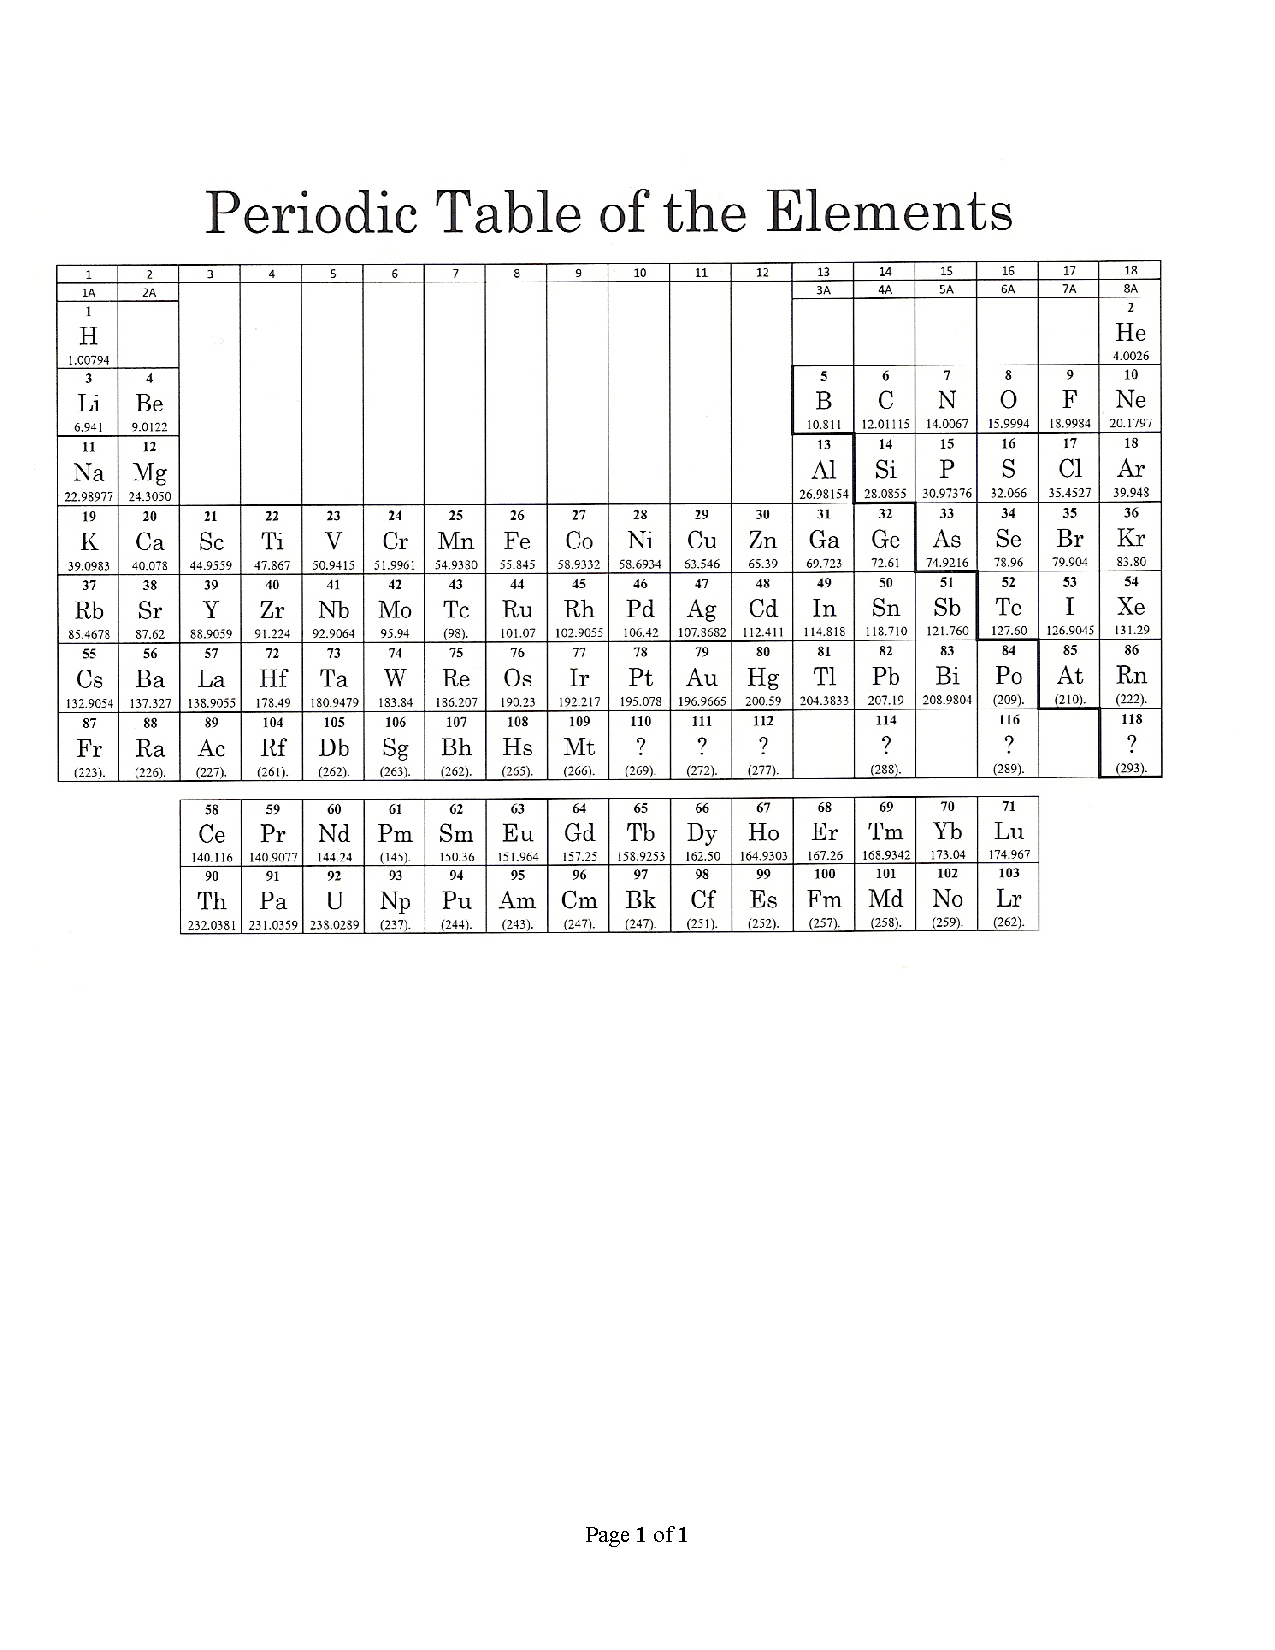
\includepdf[pages={-}]{Periodic Table for testing.pdf}


\end{document}